% The fucking story

% those people before me thought you the basics about the standard and the protocol and
% how we extract useful information out of the telegrams

% in thematical order
% - what is the current scale of operation
%   - map of stations
%   - plot
%   - with which receivers
% - how do we process data
%   - accurate: radio + telegram decoder
%   - services: just {
%   - lessons learned
% - what do you can get from us
% - what do we achieve examplary calculation
  % - but you can help increase quality as segway into

% =================================================

\usetikzlibrary{calc}
\usetikzlibrary{decorations.pathreplacing,decorations.markings,shapes.geometric}
\tikzset{radiation/.style={{decorate,decoration={expanding waves,angle=90,segment length=4pt}}}}

\lstdefinelanguage{Nix}{
  keywords={true, false},
  keywordstyle=\color{blue}\bfseries,
  ndkeywords={class, export, boolean, throw, implements, import, this},
  ndkeywordstyle=\small \color{darkgray}\bfseries,
  identifierstyle=\scriptsize \color{black},
  sensitive=false,
  comment=[l]{//},
  morecomment=[s]{/*}{*/},
  commentstyle=\color{purple}\ttfamily,
  stringstyle=\color{red}\ttfamily,
  morestring=[b]',
  morestring=[b]",
  basicstyle=\scriptsize,
  %$numbers=left,
  stepnumber=1,
  numbersep=8pt,
  tabsize=4,
  showspaces=false,
  showstringspaces=false
}

\begin{frame}
  \frametitle{Receivers in Operation}

\begin{figure}
\begin{columns}
\column{.5\linewidth}
\centering
  \includegraphics[height=0.65\textheight]{figs/map_dresden.jpg}
  \caption{Receivers in Dresden}
\column{.5\linewidth}
\centering
  \includegraphics[height=0.65\textheight]{figs/map_chemnitz.jpg}
  \caption{Receivers in Chemnitz}
\end{columns}
\end{figure}

\end{frame}

% =================================================

\begin{frame}
\frametitle{Received Data}

\begin{figure}[h!]
  \begin{center}
    \begin{tikzpicture}[scale=0.6]
      \begin{axis}[
          width=\linewidth,
          grid=major,
          grid style={dashed,gray!30},
          xlabel=Time over 4 days,
          ylabel=Telegrams in 5 minute intervals,
          %x unit=time,
          %y unit=\si{\ampere},
          %legend style={at={(0.5,-0.2)},anchor=north},
          x tick label style={rotate=90,anchor=east},
          xticklabels={,,},
          %xticklabels={day1, day2, day3, day4} TODO: make nice labels
        ]
        \addplot
        table[x=time,y=value,col sep=comma] {figs/rawdata.csv};
      \end{axis}
    \end{tikzpicture}
  \end{center}
\end{figure}


\end{frame}

% =================================================

\begin{frame}
\frametitle{What can we see}

\begin{figure}[h!]
  \begin{center}
    \missingfigure[figwidth=6cm]{Heat Map of Locations}
    \caption{visible reporting points in the city}
  \end{center}
\end{figure}


\end{frame}

% =================================================

\begin{frame}
\frametitle{Converage Estimation}

\begin{figure}
\begin{columns}
\column{.5\linewidth}
\begin{center}
  \includegraphics[height=0.6\textheight]{figs/urbic_stops_dresden.jpg}
  \caption{Statistic of traffic lights in dresden from \Colorhref{https://urbic-system.com/wp-content/uploads/2020/10/Qualitaetssicherung-an-Lichtsignalanlagen-aus-Sicht-des-OEPNV-im-urbanen-Umfeld-Kopie.pdf}{urbic 01/2014}}
\end{center}
\column{.5\linewidth}
\raggedright
\vspace{0.5cm}

\begin{itemize}
  \item \todo[inline]{Add query}
  \item See $\approx$ 60\% of the city
\end{itemize}

\end{columns}
\end{figure}

\end{frame}

% =================================================

\begin{frame}
\frametitle{Assembeling a Receiver}

\begin{figure}
\begin{columns}
\column{.5\linewidth}
\begin{center}
\includegraphics[height=0.7\textheight]{figs/station_barkhausen.jpg}
\end{center}
\column{.5\linewidth}
\raggedright
\caption{\raggedright Station Barkhausenbau}
%\vspace{0.5cm}

\begin{itemize}
	%\item\todo[inline]{make caption allign left}
	%\item\todo[inline]{please provide some details about this station}
  \item GDR powersuply casing (10\euro)
  \item Dell Wyse 3040 (70\euro)
  \item Rad1o Badge (e.g RTL SDR 30\euro)
  \item Hardware Filter (20\euro)
  \item Antenna (15\euro)
  \item Miscellaneous items (15\euro)
  \item Healthy amounts of kapton
\end{itemize}

$\Rightarrow$ ~160\euro \ per Station

\end{columns}
\end{figure}

\end{frame}

% =================================================

\begin{frame}
\frametitle{Receiver}

\begin{figure}
\begin{columns}
\column{.5\linewidth}
\begin{center}
  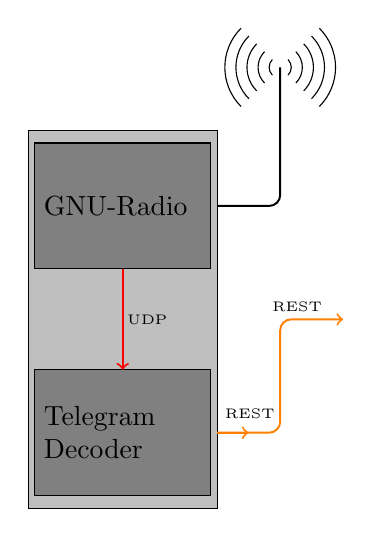
\begin{tikzpicture}[scale=0.8]
    % Station Box
\filldraw[draw=black,fill=lightgray] (0,3) rectangle (3,-3);

% GNU Radio and Telegram Decoder
\filldraw[draw=black,fill=gray] (0.1,0.8) rectangle (2.9,2.8);
\filldraw[draw=black,fill=gray] (0.1,-0.8) rectangle (2.9,-2.8);

% Data Flow
\draw[->,rounded corners, line width=0.25mm, red] (1.5, 0.8) -- (1.5,-0.8);
\draw[->,rounded corners, line width=0.25mm, orange] (3, -1.8)  -- (4,-1.8) -- (4,0) -- (5, 0);

% Antenna Drawing
\draw[rounded corners, line width=0.25mm, black] (3, 1.8) -- (4,1.8) -- (4, 4);
\draw[radiation,decoration={angle=45}] (4,4) -- +(180:1);
\draw[radiation,decoration={angle=45}] (4,4) -- +(0:1);

% Labeling
\node[text width=2cm] at (1.5,1.8) {GNU-Radio};
\node[text width=2cm] at (1.5,-1.8) {\centering Telegram Decoder};


\node[text width=0.2cm] at (4,0.2) {\tiny REST};
\node[text width=0.2cm] at (1.7,0) {\tiny UDP};

    \node[text width=0.2cm] at (3.25,-1.5) {\tiny REST};
    \draw[->,rounded corners, line width=0.25mm, orange] (3, -1.8)  -- (3.5, -1.8);

  \end{tikzpicture}
\end{center}
\column{.5\linewidth}
\raggedright
\vspace{0.5cm}

\begin{itemize}
  \item Region specific encoding depending on special quirks from the city
  \item Currently only parses R09.16 and everything else is recorded as raw-telegram
  \item Authenticates with station UUID and token
\end{itemize}

\end{columns}
\end{figure}

\end{frame}

% =================================================

\begin{frame}
  \frametitle{Server}
  \begin{figure}
    \begin{center}
      \begin{tikzpicture}[thick,scale=0.85, every node/.style={scale=0.85}]
        \filldraw[draw=black,fill=lightgray] (5,3) rectangle (19,-3);

\filldraw[draw=black,fill=gray] (5.5,1) rectangle (9,-1);
\node[database,label=above:postgres,database radius=0.7cm,database segment height=0.35cm] at (10,-2) {};
\node[database,label=above:stops.json,database radius=0.7cm,database segment height=0.35cm] at (10,0.5) {};

% DataAccm <-> Postgres
\draw[->,rounded corners, line width=0.25mm] (6, -1)  -- (6,-2) -- (9.2,-2);
\draw[->,rounded corners, line width=0.25mm] (9.2, -1.9)  -- (6.1,-1.9) -- (6.1,-1);

% User Facing Services
\filldraw[draw=black,fill=gray] (15,2.9) rectangle (18.5,1.6);
\filldraw[draw=black,fill=gray] (15,1.4) rectangle (18.5,0.1);
\filldraw[draw=black,fill=gray] (15,-0.1) rectangle (18.5,-1.4);
\filldraw[draw=black,fill=gray] (15,-1.6) rectangle (18.5,-2.9);

% GRPC Arrows
\draw[->,rounded corners, red, line width=0.25mm] (6, 1)  -- (6,2.25) -- (15,2.25);
\draw[->,rounded corners, red, line width=0.25mm] (12.7, 2.25)  -- (12.7,0.9) -- (15,0.9);

% Postgres Arrows
% Tracy
\draw[->,rounded corners, line width=0.25mm] (10.8, -2.2)  -- (15,-2.2);
\draw[->,rounded corners, line width=0.25mm] (15, -2.3)  -- (10.8,-2.3);
% Clicky-Bunty-Server
\draw[->,rounded corners, line width=0.25mm] (15, -0.8)  -- (12.9, -0.8) -- (12.9, -2.1) -- (10.8,-2.1);
\draw[->,rounded corners, line width=0.25mm] (10.8, -2)  -- (12.8, -2) -- (12.8, -0.7) -- (15,-0.7);
% DVB-API
\draw[->,rounded corners, line width=0.25mm] (10.8, -1.9)  -- (12.7, -1.9) -- (12.7, 0.6) -- (15, 0.6);

% Labeling
\node[text width=3cm] at (7.3,0) {Data-Accumulator};
\node[text width=1cm] at (16.75,2.25) {Funnel};
\node[text width=2cm] at (16.8,0.75) {DVB-API};
\node[text width=2.5cm] at (16.8,-0.75) {Clicky-Bunty};
\node[text width=1cm] at (16.75,-2.25) {Tracy};

% Look Ups
\draw[->,rounded corners, black!60!green, line width=0.25mm] (10.8, 0.75)  -- (15, 0.75);

% Labeling Arrows
\node[text width=2cm] at (11.7,2.5) {\tiny GRPC/Protobuf};
\node[text width=1cm] at (11.7,1) {\tiny Look UP};
\node[text width=1cm] at (11.7, -1.7) {\tiny Queries};

\draw[->,rounded corners, black!30!orange, line width=0.25mm] (4.75, 0)  -- (5.5, 0);

      \end{tikzpicture}
    \end{center}
  \end{figure}
\end{frame}

% =================================================

\begin{frame}
\frametitle{Architecture}

% Funnel
% DVB-API
% Clicky-Bunty
% Tracy
\begin{tikzpicture}[thick,scale=0.55, every node/.style={scale=0.65}]

% Station Box
\filldraw[draw=black,fill=lightgray] (0,3) rectangle (3,-3);

% GNU Radio and Telegram Decoder
\filldraw[draw=black,fill=gray] (0.1,0.8) rectangle (2.9,2.8);
\filldraw[draw=black,fill=gray] (0.1,-0.8) rectangle (2.9,-2.8);

% Data Flow
\draw[->,rounded corners, line width=0.25mm, red] (1.5, 0.8) -- (1.5,-0.8);
\draw[->,rounded corners, line width=0.25mm, orange] (3, -1.8)  -- (4,-1.8) -- (4,0) -- (5, 0);

% Antenna Drawing
\draw[rounded corners, line width=0.25mm, black] (3, 1.8) -- (4,1.8) -- (4, 4);
\draw[radiation,decoration={angle=45}] (4,4) -- +(180:1);
\draw[radiation,decoration={angle=45}] (4,4) -- +(0:1);

% Labeling
\node[text width=2cm] at (1.5,1.8) {GNU-Radio};
\node[text width=2cm] at (1.5,-1.8) {\centering Telegram Decoder};


\node[text width=0.2cm] at (4,0.2) {\tiny REST};
\node[text width=0.2cm] at (1.7,0) {\tiny UDP};

\filldraw[draw=black,fill=lightgray] (5,3) rectangle (19,-3);

\filldraw[draw=black,fill=gray] (5.5,1) rectangle (9,-1);
\node[database,label=above:postgres,database radius=0.7cm,database segment height=0.35cm] at (10,-2) {};
\node[database,label=above:stops.json,database radius=0.7cm,database segment height=0.35cm] at (10,0.5) {};

% DataAccm <-> Postgres
\draw[->,rounded corners, line width=0.25mm] (6, -1)  -- (6,-2) -- (9.2,-2);
\draw[->,rounded corners, line width=0.25mm] (9.2, -1.9)  -- (6.1,-1.9) -- (6.1,-1);

% User Facing Services
\filldraw[draw=black,fill=gray] (15,2.9) rectangle (18.5,1.6);
\filldraw[draw=black,fill=gray] (15,1.4) rectangle (18.5,0.1);
\filldraw[draw=black,fill=gray] (15,-0.1) rectangle (18.5,-1.4);
\filldraw[draw=black,fill=gray] (15,-1.6) rectangle (18.5,-2.9);

% GRPC Arrows
\draw[->,rounded corners, red, line width=0.25mm] (6, 1)  -- (6,2.25) -- (15,2.25);
\draw[->,rounded corners, red, line width=0.25mm] (12.7, 2.25)  -- (12.7,0.9) -- (15,0.9);

% Postgres Arrows
% Tracy
\draw[->,rounded corners, line width=0.25mm] (10.8, -2.2)  -- (15,-2.2);
\draw[->,rounded corners, line width=0.25mm] (15, -2.3)  -- (10.8,-2.3);
% Clicky-Bunty-Server
\draw[->,rounded corners, line width=0.25mm] (15, -0.8)  -- (12.9, -0.8) -- (12.9, -2.1) -- (10.8,-2.1);
\draw[->,rounded corners, line width=0.25mm] (10.8, -2)  -- (12.8, -2) -- (12.8, -0.7) -- (15,-0.7);
% DVB-API
\draw[->,rounded corners, line width=0.25mm] (10.8, -1.9)  -- (12.7, -1.9) -- (12.7, 0.6) -- (15, 0.6);

% Labeling
\node[text width=3cm] at (7.3,0) {Data-Accumulator};
\node[text width=1cm] at (16.75,2.25) {Funnel};
\node[text width=2cm] at (16.8,0.75) {DVB-API};
\node[text width=2.5cm] at (16.8,-0.75) {Clicky-Bunty};
\node[text width=1cm] at (16.75,-2.25) {Tracy};

% Look Ups
\draw[->,rounded corners, black!60!green, line width=0.25mm] (10.8, 0.75)  -- (15, 0.75);

% Labeling Arrows
\node[text width=2cm] at (11.7,2.5) {\tiny GRPC/Protobuf};
\node[text width=1cm] at (11.7,1) {\tiny Look UP};
\node[text width=1cm] at (11.7, -1.7) {\tiny Queries};

\draw[->,rounded corners, black!30!orange, line width=0.25mm] (4.75, 0)  -- (5.5, 0);


% Station Box
\filldraw[draw=black,fill=lightgray] (21,3) rectangle (24,-3);

% GNU Radio and Telegram Decoder
\filldraw[draw=black,fill=gray] (21.1,0.1) rectangle (23.9,2.9);
\filldraw[draw=black,fill=gray] (21.1,-0.1) rectangle (23.9,-1.4);
\filldraw[draw=black,fill=gray] (21.1,-1.6) rectangle (23.9,-2.9);

% Labeling
\node[text width=2cm] at (23,1.5) {Map};
\node[text width=2cm] at (23,-0.75) {Click};
\node[text width=2cm] at (23,-2.25) {Tracy};

\draw[->,rounded corners, black!30!orange, line width=0.25mm] (18.5, 2.25)  -- (21, 2.25);
\draw[->,rounded corners, black!30!orange, line width=0.25mm] (18.5, 0.75)  -- (21, 0.75);

\draw[->,rounded corners, black!30!orange, line width=0.25mm] (21, -0.7)  -- (18.5, -0.7);
\draw[->,rounded corners, black!30!orange, line width=0.25mm] (18.5, -0.8)  -- (21, -0.8);

\draw[->,rounded corners, black!30!orange, line width=0.25mm] (21, -2.2)  -- (18.5, -2.2);
\draw[->,rounded corners, black!30!orange, line width=0.25mm] (18.5, -2.3)  -- (21, -2.3);


\node[text width=0.1cm] at (19.5,1) {\tiny REST};
\node[text width=0.1cm] at (19.5,-2) {\tiny REST};
\node[text width=0.1cm] at (19.5,2.5) {\tiny SOCKET};
\node[text width=0.1cm] at (19.5,-0.5) {\tiny SOCKET};


\node[text width=0.2cm] at (4,0.2) {\tiny REST};
\draw[->,rounded corners, line width=0.25mm, orange] (3, -1.8)  -- (4,-1.8) -- (4,0) -- (5, 0);

\end{tikzpicture}

\end{frame}

%TODO: Friendship Ended with Influx

% =================================================

\begin{frame}
\frametitle{Throughput}

\begin{figure}[h!]
  \begin{center}
    \begin{tikzpicture}[scale=0.6]
      \begin{axis}[
          width=\linewidth,
          grid=major,
          grid style={dashed,gray!30},
          xlabel=Benchmark over 5 mins,
          ylabel=Telegrams per Second,
          %x unit=time,
          %y unit=\si{\ampere},
          %legend style={at={(0.5,-0.2)},anchor=north},
          x tick label style={rotate=90,anchor=east},
          xticklabels={,,},
          %xticklabels={day1, day2, day3, day4} TODO: make nice labels
        ]
        \addplot
        table[x=time,y=send,col sep=comma] {figs/benchmark.csv};
        \addplot
        table[x=time,y=receive,col sep=comma,color=red] {figs/benchmark.csv};
      \end{axis}
    \end{tikzpicture}
  \end{center}
\end{figure}


\end{frame}

% =================================================

\begin{frame}
  \frametitle{Technical Loans}
  \framesubtitle{Lessons Learned}

\begin{figure}
\begin{columns}
\column{.5\linewidth}
\begin{center}
\includegraphics[height=0.65\textheight]{figs/meme_postgres_influx.png}
\end{center}
\column{.5\linewidth}
\raggedright
\vspace{0.5cm}

\begin{itemize}
  \item Influx
        \begin{itemize}
          \item Database dumps costs 14GB of RAM
          \item Server died hourly
        \end{itemize}
    \item Single point of truth
    \begin{itemize}
        \item Implement Protocols in Libraries which is then used by both parties.
    \end{itemize}
    \item Hardware homogenity
\end{itemize}
\end{columns}
\end{figure}

\end{frame}

% =================================================

\begin{frame}[fragile]
\frametitle{Data We Currently Provide}
\framesubtitle{Funnel: Websocket}
\begin{figure}
\begin{columns}
  \column{.5\linewidth}
  \includegraphics[height=0.65\textheight]{figs/data_dump.png}
\column{.5\linewidth}
\raggedright
\vspace{0.5cm}

\begin{itemize}
  \item 7.7 million telegrams are already recorded
  \item hourly and daily dumps can be fetched from \url{https://files.dvb.solutions}
\end{itemize}
\end{columns}
\end{figure}
\end{frame}
% =================================================

\begin{frame}[fragile]
\frametitle{Data we Currently Provide}
\framesubtitle{Funnel: Websocket}
\begin{figure}
\begin{columns}
  \column{.5\linewidth}
\begin{lstlisting}[basicstyle=\scriptsize]
{
  "time":1662932144,
  "station":"97d028ec-43e2-4473-...",
  "region":0,
  "telegram_type":16,
  "reporting_point":8366,
  "junction":209,
  "direction":1,
  "request_status":2,
  "delay":0,
  "priority":0,
  "direction_request":0,
  "line":4,
  "run_number":9,
  "destination_number":31,
  "train_length":0
}
\end{lstlisting}
\column{.5\linewidth}
\raggedright
\vspace{0.5cm}

\begin{itemize}
  \item \url{https://socket.dvb.solutions}
  \item Configurable Filters (region, line, junction)
  \item Deduplicated
  \item Very raw
\end{itemize}
\end{columns}
\end{figure}
\end{frame}

% =================================================

\begin{frame}[fragile]
\frametitle{Data We Currently Provide}
\framesubtitle{stop.json \& graph.json}

  \begin{itemize}
    \item \url{https://map.dvb.solutions/stop/<region id>.json}
    \item \url{https://map.dvb.solutions/stop/all.json}
    \item \url{https://map.dvb.solutions/graph/<region id>.json}
    \item \url{https://map.dvb.solutions/graph/all.json}
  \end{itemize}
\end{frame}
% =================================================

\begin{frame}[fragile]
\frametitle{Data We Currently Provide}
\framesubtitle{REST DVB-API}

\begin{itemize}
     \item \url{https://api.dvb.solutions}
     \item \textbf{GET  /vehicles/0/all}
     \item \textbf{POST /vehicles/0/query}
     \item \textbf{POST /network/0/estimated\_travel\_time}
     \item \textbf{POST /static/0/coordinates}
  \end{itemize}
\end{frame}

% =================================================
